\part{Ověření správnosti korespondencí}	
	
	Máme k dispozici algoritmy, pomocí kterých jsme schopni nalézt korespondující svazky. U~některých, zvlášť u algoritmů v kapitole  \ref{sec: korespondence_ocasky} a \ref{sec: poloha_tok}, můžeme kromě správných korespondencí nalézt řadu falešných  dvojic svazků.
	
	Chceme nalézt metodu schopnou rozhodnout, zda jsou korespondence správné či nesprávné. 
	\vspace{4mm}
	
\section{Množiny korespondencí}
Přicházíme s nápadem rozdělit množiny na čtyři disjunktní množiny.

	\begin{itemize}
	\item \textbf{Optimalizované} -  Do množiny optimalizovaných korespondencí patří korespondence, o kterých jsme si velmi jisti, že jsou správné. Tato množina korespondencí určuje model kamene. 
	
	\item \textbf{Kriteriální} - Kriteriální množina korespondencí složí k výpočtu hodnotícího kritéria. Do této množiny patří, stejně jako do množiny optimalizovaných korespondencí, spolehlivě určitelné korespondence.  
	
	\item \textbf{Kandidátské} - Korespondence, o kterých chceme rozhodnout, zda jsou či nejsou správné.  
	
	\item \textbf{Ostatní} - Korespondence nehodící se ani do jedné z předchozích množin. Typicky svazky příliš vzdálené a svazky s nízkým zářivým tokem.  
\end{itemize}		
	
\section{Rozhodovací algoritmus}
	Množina optimalizovaných korespondencí určujme model kamene. Pro tento model je pro kriteriální množinu korespondencí vypočítáno optimalizační kritérium z rovnice \ref{eq: opt_criter} (dále pouze jako \textit{kritérium}) a určen jeho součet $\varepsilon_0 = \sum\vec{\varepsilon}$.
	 
	Vybereme jednu korespondenci z množiny kandidátů a přidáme ji do množiny optimalizovaných korespondencí. Podle množiny optimalizovaných korespondencí odhadneme nový model kamene. Na tomto modelu  vypočítáme srovnávací \textit{kritérium} pro množinu kriteriálních korespondencí $\varepsilon_c = \sum\vec{\varepsilon}$. 
	
	Změna optimalizačního kritéria je potom 
	
	\begin{equation}
	\Delta\varepsilon  = \varepsilon_0 - \varepsilon_c\,.
	\end{equation}
	
	Pokud je $\Delta\varepsilon  > \varepsilon_t$, kde $\varepsilon_t$ je rozhodovací práh, prohlásíme tuto korespondenci za správnou a ponecháme v množině optimalizovaných korespondencí. V opačném případě korespondenci odstraníme.
	
	Čekali bychom, že optimální práh $\varepsilon_t$ by mohl být roven nule. Po přidání správné korespondence do množiny optimalizovaných bude  $\varepsilon_0 > \varepsilon_c$ a pokud přidáme falešnou korespondenci, tak $\varepsilon_0 < \varepsilon_c$. 

\section{Simulace dat}
\label{sec: sber dat}
	Pro ověření vhodnosti metody použijeme simulační programu LADOK. 	
	
	Vytvoříme ideální model kamene \textit{viva12}. Změníme náhodně náklon faset ideálního modelu a z faset vytvoříme \textit{deformovaný} model kamene. Změna náklonu je náhodně vybrána z normálního rozdělení se střední hodnotou $\mu = 0$ a směrodatnou odchylkou $\sigma = $ \SI{0.5}{\degree}. 
	
	 Pro \textit{deformovaný} model vypočítáme pomocí programu LADOK výstupní svazky s maximálně 11-ti dopadovými fasetami. Svazky promítneme do obrazu. Pozici svazků v obraze zašumíme náhodným výběrem z normálního rozdělení se střední hodnotou $\mu = 0$ a směrodatnou odchylkou, která odpovídá polovině maximální citlivosti dopadových faset svazku výstupního úhlu. Odrazová faseta má citlivost 2. U lomu za citlivost fasety dosazujeme $\dfrac{\mathrm{d}\alpha_2}{\mathrm{d}\alpha_1}$ z rovnice \ref{eq:derivace uhlu} tj. změnu lomeného úhlu $\alpha_2$ na změně úhlu dopadu $\alpha_1$ (kapitola \ref{sec: zmena smeru}). Zašuměné pozice svazků představují simulaci pozorovaných svazků.  
	 
	Vybereme korespondence do optimalizované množiny korespondencí. Podle množiny optimalizovaných korespondencí optimalizujeme kámen a dostaneme referenční optimalizovaný model. 
	
	Zvolíme množinu kriteriálních korespondencí a vypočítáme $\varepsilon_0$. 
	
	Vybereme množinu kandidátských korespondencí a ke každému kandidátovi nalezneme podle kritéria $\mathbf{L}$ z rovnice  \ref{eq: L_tok} nejbližší nesprávnou korespondenci. 
	
	Do optimalizované množiny přidáváme jednotlivě správné či nesprávné kandidátské korespondence. Podle rozšířené množiny optimalizovaných korespondencí optimalizujeme sklon faset kamene, určíme $\varepsilon_c$ a následně $\Delta\varepsilon$.   	
	
	Metoda předpokládá, že po optimalizaci se model nezmění natolik, aby se mohly zaniknout některé svazky, obsaženy v  množině kriteriálních korespondencí. 		

\section{Oddělitelnost}
	Ke každé správné kandidátské korespondenci máme určenou jednu špatnou. Počet správných a špatných korespondencí je stejný a je roven $n_c$. 

	Máme daný rozhodovací práh $\varepsilon_{t_0}$.	Číslo $n_t$ určuje počet správných korespondencí, pro které $\Delta\varepsilon  < \varepsilon_{t_0}$ a $n_f$ počet falešných korespondencí s $\Delta\varepsilon  > \varepsilon_{t_0}$. 
	
	Potom oddělitelnost definujeme jako 
	
	\begin{equation}
		S = 1 - \frac{1}{2} \cdot \frac{n_t+n_f}{n_c}\,. 
	\label{eq: S}
	\end{equation}
	
	Z rovnice \ref{eq: S} je zřejmé, že $S \in \left\langle0,\,1 \right\rangle$ a v ideálním případě, kdy prahem oddělíme všechny správné a špatné korespondence, je $S$ rovno 1. Optimální práh $\varepsilon_{t}$ určujeme pro $S$ maximální. Oddělitelnosti kandidátských korespondencí budeme dále uvažovat pouze pro optimální práh. 
	
	 
\section{Rozdělení svazků do množin}

Množiny optimalizovaných a kriteriálních korespondencí jsme se rozhodli sestavit z korespondencí deseti tříd \textbf{1A}, \textbf{3A}, \textbf{6A}, \textbf{6B}, \textbf{6C}, \textbf{6D}, \textbf{7A}, \textbf{7B}, \textbf{8A} a \textbf{9A}. Korespondence svazků třídy \textbf{1A} a \textbf{3A} nalezneme spolehlivě (kapitoly \ref{sec: 1A} a \ref{sec:3A}). 

Svazky tříd \textbf{6A}, \textbf{6B}, \textbf{6C}, \textbf{6D}, \textbf{7A} a \textbf{7B} dobře určují ocásky a zářivý tok. Jejich korespondence jsou s vysokou pravděpodobností správné. 

Hustota ostatních svazků v blízkém okolí svazků tříd \textbf{8A} a \textbf{9A} je nízká, proto pro mě snadněji nalezneme korespondující svazky. 

V době, kdy jsme testovali tuto metodu, jsme nebyli schopni spolehlivě nalézt korespondence svazků třídy \textbf{5D}. Sběr dat je extrémně časově náročný, proto jsme tuto třídu zařadili pouze do množiny kriteriálních korespondencí. Kriteriální množina obsahuje dalších 26 tříd svazků, které lze často detekovat v našich experimentech a mají ve své cestě maximálně 9 dopadových faset. 


\section{Vhodné zvolení optimalizační a kriteriální množiny}
\label{sec: vhodnostOpt}
	Připravili jsme experiment hodnotící vhodnost kombinace tříd svazků v optimalizované a kriteriální množině. Máme na výběr z 10-ti tříd. Pokud chceme, aby v každé množině byla alespoň jedna třída svazků, dostaneme 1022 možných kombinací. Pro tolik kombinací nejsme z časového omezení schopni provést dostatečný počet výpočtů, abychom mohli zjistit, která z kombinací je nejvhodnější. 

	Počet kombinací omezíme. Množina optimalizovaných korespondencí bude obsahovat 6 tříd svazků a kriteriální množina zbývající 4 třídy svazků. Optimalizované korespondence vybereme tak, abychom zajistili, že optimalizační úloha bude dobře podmíněna a my bychom mohli při optimalizaci uvolnit všechny fasety. V optimalizační množině tak bude  minimálně jedna třída z dvojice tříd \textbf{1A} a \textbf{3A}, minimálně 3 třídy ze čtveřice \textbf{6A}, \textbf{6B}, \textbf{6C} a \textbf{6D} a minimálně minimálně jedna ze čtveřice \textbf{7A}, \textbf{7B}, \textbf{8A} a \textbf{9A}. Tímto způsobem je možné sestavit 72 kombinací optimalizované a kriteriální množiny. 
	
	Data sbíráme podle bodu \ref{sec: sber dat}. Jeden stejný \textit{deformovaný} model a simulované měřené svazky použijeme pro všechny možné kombinace optimalizované a kriteriální množiny. Pro každou kombinaci získáme hodnoty $\Delta\varepsilon$ pro správné a špatné korespondence a určíme oddělitelnost $S$. Po výpočtu pro všechny kombinace vypočítáme nový \textit{deformovaný} model a simulované měřené svazky a výpočet opakujeme. 
	
	Celkem jsme provedli výpočet pro 10 \textit{deformovaných} modelů a dostali 10 hodnot $S$ pro každou kombinaci. Při použití procesoru o frekvenci \SI{2.4}{\giga\Hz} je doba výpočtu přibližně 42 dní. 
	
	Střední hodnota $S$ pro jednotlivé kombinace je zapsána v tabulkách \ref{table: MeanSeperability1} a \ref{table: MeanSeperability2} a znázorněna v grafu \ref{fig: oddelitelnost}. Mezi výslednými hodnotami $S$ není u jednotlivých korespondencí výrazný rozdíl. Z tabulky lze vypozorovat, že korespondence třídy\textbf{1A} je dobré umístit do optimalizované množiny a třídu \textbf{3A} do množiny kriteriálních korespondencí. Nejméně vhodná se zdá kombinace č. 47.  
	
\begin{table}[h!]
\centering
\scalebox{0.97}{
\begin{tabular}{|c||c|c|c|c|c|c||c|c|c|c||c|}
\hline
Kombinace č. &  \multicolumn{6}{l||}{Optimalizační množina} & \multicolumn{4}{l||}{Kriteriální množina} & $S$ \\
\hline \hline 
\textbf{38} & 1A & 6A & 6C & 6D & 8A & 9A & 3A & 6B & 7A & 7B & 0.853 \\
\hline
\textbf{20} & 1A & 6A & 6B & 6C & 6D & 9A & 3A & 7A & 7B & 8A & 0.849 \\
\hline
\textbf{26} & 1A & 6A & 6B & 6C & 8A & 9A & 3A & 6D & 7A & 7B & 0.847 \\
\hline
\textbf{24} & 1A & 6A & 6B & 6C & 7B & 8A & 3A & 6D & 7A & 9A & 0.846 \\
\hline
\textbf{34} & 1A & 6A & 6C & 6D & 7A & 8A & 3A & 6B & 7B & 9A & 0.845 \\
\hline
\textbf{40} & 1A & 6B & 6C & 6D & 7A & 8A & 3A & 6A & 7B & 9A & 0.844 \\
\hline
\textbf{32} & 1A & 6A & 6B & 6D & 8A & 9A & 3A & 6C & 7A & 7B & 0.844 \\
\hline
\textbf{30} & 1A & 6A & 6B & 6D & 7B & 8A & 3A & 6C & 7A & 9A & 0.842 \\
\hline
\textbf{36} & 1A & 6A & 6C & 6D & 7B & 8A & 3A & 6B & 7A & 9A & 0.841 \\
\hline
\textbf{41} & 1A & 6B & 6C & 6D & 7A & 9A & 3A & 6A & 7B & 8A & 0.841 \\
\hline
\textbf{42} & 1A & 6B & 6C & 6D & 7B & 8A & 3A & 6A & 7A & 9A & 0.840 \\
\hline
\textbf{18} & 1A & 6A & 6B & 6C & 6D & 7B & 3A & 7A & 8A & 9A & 0.840 \\
\hline
\textbf{11} & 1A & 3A & 6A & 6C & 6D & 8A & 6B & 7A & 7B & 9A & 0.840 \\
\hline
\textbf{10} & 1A & 3A & 6A & 6C & 6D & 7B & 6B & 7A & 8A & 9A & 0.840 \\
\hline
\textbf{64} & 3A & 6A & 6C & 6D & 7B & 8A & 1A & 6B & 7A & 9A & 0.839 \\
\hline
\textbf{22} & 1A & 6A & 6B & 6C & 7A & 8A & 3A & 6D & 7B & 9A & 0.839 \\
\hline
\textbf{66} & 3A & 6A & 6C & 6D & 8A & 9A & 1A & 6B & 7A & 7B & 0.839 \\
\hline
\textbf{33} & 1A & 6A & 6C & 6D & 7A & 7B & 3A & 6B & 8A & 9A & 0.838 \\
\hline
\textbf{44} & 1A & 6B & 6C & 6D & 8A & 9A & 3A & 6A & 7A & 7B & 0.838 \\
\hline
\textbf{28} & 1A & 6A & 6B & 6D & 7A & 8A & 3A & 6C & 7B & 9A & 0.838 \\
\hline
\textbf{13} & 1A & 3A & 6B & 6C & 6D & 7A & 6A & 7B & 8A & 9A & 0.838 \\
\hline
\textbf{2} & 1A & 3A & 6A & 6B & 6C & 7B & 6D & 7A & 8A & 9A & 0.837 \\
\hline
\textbf{4} & 1A & 3A & 6A & 6B & 6C & 9A & 6D & 7A & 7B & 8A & 0.837 \\
\hline
\textbf{12} & 1A & 3A & 6A & 6C & 6D & 9A & 6B & 7A & 7B & 8A & 0.836 \\
\hline
\textbf{16} & 1A & 3A & 6B & 6C & 6D & 9A & 6A & 7A & 7B & 8A & 0.836 \\
\hline
\textbf{6} & 1A & 3A & 6A & 6B & 6D & 7B & 6C & 7A & 8A & 9A & 0.836 \\
\hline
\textbf{39} & 1A & 6B & 6C & 6D & 7A & 7B & 3A & 6A & 8A & 9A & 0.836 \\
\hline
\textbf{27} & 1A & 6A & 6B & 6D & 7A & 7B & 3A & 6C & 8A & 9A & 0.835 \\
\hline
\textbf{69} & 3A & 6B & 6C & 6D & 7A & 9A & 1A & 6A & 7B & 8A & 0.834 \\
\hline
\textbf{7} & 1A & 3A & 6A & 6B & 6D & 8A & 6C & 7A & 7B & 9A & 0.834 \\
\hline
\textbf{9} & 1A & 3A & 6A & 6C & 6D & 7A & 6B & 7B & 8A & 9A & 0.834 \\
\hline
\textbf{14} & 1A & 3A & 6B & 6C & 6D & 7B & 6A & 7A & 8A & 9A & 0.834 \\
\hline
\textbf{17} & 1A & 6A & 6B & 6C & 6D & 7A & 3A & 7B & 8A & 9A & 0.834 \\
\hline
\textbf{56} & 3A & 6A & 6B & 6D & 7A & 8A & 1A & 6C & 7B & 9A & 0.833 \\
\hline
\textbf{37} & 1A & 6A & 6C & 6D & 7B & 9A & 3A & 6B & 7A & 8A & 0.833 \\
\hline
\textbf{58} & 3A & 6A & 6B & 6D & 7B & 8A & 1A & 6C & 7A & 9A & 0.833 \\
\hline
\textbf{60} & 3A & 6A & 6B & 6D & 8A & 9A & 1A & 6C & 7A & 7B & 0.833 \\
\hline
\textbf{25} & 1A & 6A & 6B & 6C & 7B & 9A & 3A & 6D & 7A & 8A & 0.832 \\
\hline
\textbf{43} & 1A & 6B & 6C & 6D & 7B & 9A & 3A & 6A & 7A & 8A & 0.831 \\
\hline
\textbf{8} & 1A & 3A & 6A & 6B & 6D & 9A & 6C & 7A & 7B & 8A & 0.830 \\
\hline
\textbf{1} & 1A & 3A & 6A & 6B & 6C & 7A & 6D & 7B & 8A & 9A & 0.830 \\
\hline
\textbf{19} & 1A & 6A & 6B & 6C & 6D & 8A & 3A & 7A & 7B & 9A & 0.829 \\
\hline
\textbf{35} & 1A & 6A & 6C & 6D & 7A & 9A & 3A & 6B & 7B & 8A & 0.829 \\
\hline
\textbf{48} & 3A & 6A & 6B & 6C & 6D & 9A & 1A & 7A & 7B & 8A & 0.827 \\
\hline
\textbf{29} & 1A & 6A & 6B & 6D & 7A & 9A & 3A & 6C & 7B & 8A & 0.827 \\
\hline
\end{tabular}
}
\caption[Střední hodnota $S$ - tabulka č. 1.]{Tabulka středních hodnot oddělitelnosti $S$ pro kombinace optimalizované a kriteriální množiny č. 1.}
\label{table: MeanSeperability1}
\end{table}

\clearpage

 
 \begin{table}[h!]
\centering
\scalebox{0.97}{
\begin{tabular}{|c||c|c|c|c|c|c||c|c|c|c||c|}
\hline
Kombinace č. &  \multicolumn{6}{l||}{Optimalizační množina} & \multicolumn{4}{l||}{Kriteriální množina} & $S$ \\
\hline \hline 
\textbf{29} & 1A & 6A & 6B & 6D & 7A & 9A & 3A & 6C & 7B & 8A & 0.827 \\
\hline
\textbf{5} & 1A & 3A & 6A & 6B & 6D & 7A & 6C & 7B & 8A & 9A & 0.827 \\
\hline
\textbf{23} & 1A & 6A & 6B & 6C & 7A & 9A & 3A & 6D & 7B & 8A & 0.826 \\
\hline
\textbf{21} & 1A & 6A & 6B & 6C & 7A & 7B & 3A & 6D & 8A & 9A & 0.826 \\
\hline
\textbf{31} & 1A & 6A & 6B & 6D & 7B & 9A & 3A & 6C & 7A & 8A & 0.826 \\
\hline
\textbf{51} & 3A & 6A & 6B & 6C & 7A & 9A & 1A & 6D & 7B & 8A & 0.825 \\
\hline
\textbf{50} & 3A & 6A & 6B & 6C & 7A & 8A & 1A & 6D & 7B & 9A & 0.825 \\
\hline
\textbf{71} & 3A & 6B & 6C & 6D & 7B & 9A & 1A & 6A & 7A & 8A & 0.822 \\
\hline
\textbf{54} & 3A & 6A & 6B & 6C & 8A & 9A & 1A & 6D & 7A & 7B & 0.822 \\
\hline
\textbf{55} & 3A & 6A & 6B & 6D & 7A & 7B & 1A & 6C & 8A & 9A & 0.821 \\
\hline
\textbf{53} & 3A & 6A & 6B & 6C & 7B & 9A & 1A & 6D & 7A & 8A & 0.820 \\
\hline
\textbf{3} & 1A & 3A & 6A & 6B & 6C & 8A & 6D & 7A & 7B & 9A & 0.820 \\
\hline
\textbf{63} & 3A & 6A & 6C & 6D & 7A & 9A & 1A & 6B & 7B & 8A & 0.820 \\
\hline
\textbf{65} & 3A & 6A & 6C & 6D & 7B & 9A & 1A & 6B & 7A & 8A & 0.816 \\
\hline
\textbf{62} & 3A & 6A & 6C & 6D & 7A & 8A & 1A & 6B & 7B & 9A & 0.814 \\
\hline
\textbf{57} & 3A & 6A & 6B & 6D & 7A & 9A & 1A & 6C & 7B & 8A & 0.813 \\
\hline
\textbf{72} & 3A & 6B & 6C & 6D & 8A & 9A & 1A & 6A & 7A & 7B & 0.811 \\
\hline
\textbf{45} & 3A & 6A & 6B & 6C & 6D & 7A & 1A & 7B & 8A & 9A & 0.810 \\
\hline
\textbf{59} & 3A & 6A & 6B & 6D & 7B & 9A & 1A & 6C & 7A & 8A & 0.809 \\
\hline
\textbf{15} & 1A & 3A & 6B & 6C & 6D & 8A & 6A & 7A & 7B & 9A & 0.806 \\
\hline
\textbf{46} & 3A & 6A & 6B & 6C & 6D & 7B & 1A & 7A & 8A & 9A & 0.806 \\
\hline
\textbf{61} & 3A & 6A & 6C & 6D & 7A & 7B & 1A & 6B & 8A & 9A & 0.806 \\
\hline
\textbf{67} & 3A & 6B & 6C & 6D & 7A & 7B & 1A & 6A & 8A & 9A & 0.801 \\
\hline
\textbf{49} & 3A & 6A & 6B & 6C & 7A & 7B & 1A & 6D & 8A & 9A & 0.799 \\
\hline
\textbf{52} & 3A & 6A & 6B & 6C & 7B & 8A & 1A & 6D & 7A & 9A & 0.794 \\
\hline
\textbf{70} & 3A & 6B & 6C & 6D & 7B & 8A & 1A & 6A & 7A & 9A & 0.793 \\
\hline
\textbf{68} & 3A & 6B & 6C & 6D & 7A & 8A & 1A & 6A & 7B & 9A & 0.792 \\
\hline
\textbf{47} & 3A & 6A & 6B & 6C & 6D & 8A & 1A & 7A & 7B & 9A & 0.780 \\
\hline
\end{tabular}
}
\caption[Střední hodnota $S$ - tabulka č. 2.]{Tabulka středních hodnot oddělitelnosti $S$ pro kombinace optimalizované a kriteriální množiny č. 2.}
\label{table: MeanSeperability2}
\end{table}

\begin{figure}[h!]
\centering
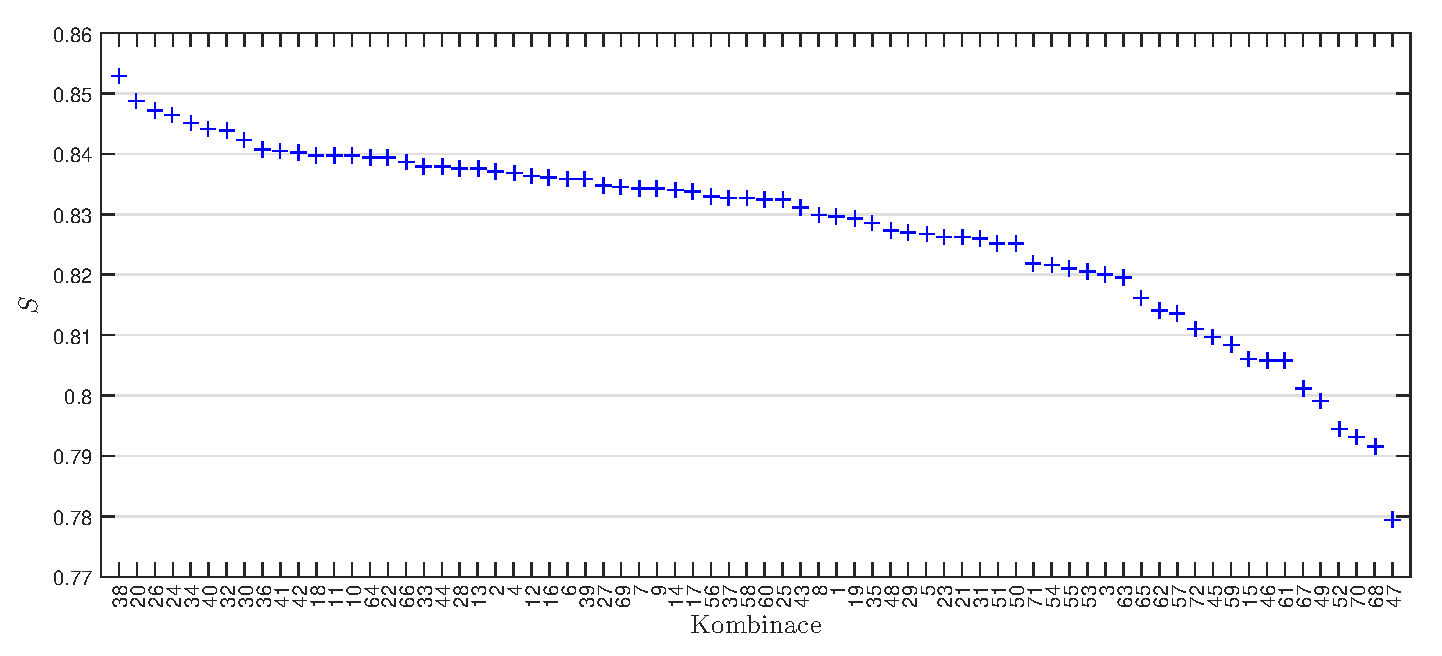
\includegraphics[width = 0.75\textwidth]{oddelitelnost.eps}
\caption[Graf oddělitelnosti $S$.]{Graf oddělitelnosti $S$ z tabulky \ref{table: MeanSeperability1} a \ref{table: MeanSeperability2}.}.
\label{fig: oddelitelnost}
\end{figure}

\clearpage

\section{Výběr kriteriální množiny}
	Data z experimentu v kapitole \ref{sec: vhodnostOpt} použijeme, abychom prozkoumali, které třídy svazků jsou vhodné pro výpočet referenčního kritéria $\varepsilon_0$.
	
	Postupujeme pro všechny jednotlivé třídy svazků. Vybereme případy, kdy daná třída svazků byla použita k výpočtu $\varepsilon_0$. Pro správné i nesprávné korespondence vypočítáme novou hodnotu $\Delta\varepsilon$, kde je kriteriální množina omezená pouze na danou třídu. Pro všechny nově vypočítané $\Delta\varepsilon$ určíme celkovou oddělitelnost $S$. Výsledky jsou znázorněny v tabulce \ref{table: GroupSeperability}. 
	
	Z výsledků vyplývá, že nejméně vhodné třídy pro zařazení do množiny kriteriálních korespondencí jsou třídy \textbf{6A} a \textbf{6B}. 

  \begin{table}[h!]
\centering
\begin{tabular}{|c||c|c|c|c|c|c|c|c|c|c|}
\hline
Třída & \textbf{1A} & \textbf{3A} & \textbf{6A}  & \textbf{6B} & \textbf{6C} & \textbf{6D} & \textbf{7A} & \textbf{7B}& \textbf{8A} & \textbf{9A}\\
\hline
$S$   &0.778 & 0.795 & 0.795 & 0.676 & 0.644 & 0.791 & 0.794 & 0.793 & 0.716 & 0.804 \\
\hline
\end{tabular}
\caption{Tabulka oddělitelnosti $S$ pro třídy svazků v kriteriální množině.}
\label{table: GroupSeperability}
\end{table}

\subsection{Výběr množiny kandidátů }
	K nejzajímavějším výsledkům se dostaneme pokud se podíváme na výsledky z hlediska vhodnosti třídy svazků v kandidátské množině. 
	
	Postupujeme jednotlivě pro třídy svazků v kandidátské množině. Vezmeme data z experimentu \ref{sec: vhodnostOpt} a vybereme pouze taková $\Delta\varepsilon$, která odpovídají dané třídě svazků.
	
	 Opět tedy dostaneme data s $\Delta\varepsilon$ pro správné a špatné korespondence, ze kterých spočítáme oddělitelnost $S$. Nyní jsou tyto data rozděleny podle tříd svazků v množině kriteriálních korespondencí. 
	 
	 Velikosti $S$  pro jednotlivé třídy svazků jsou zapsány v tabulce \ref{table: CritSeperability}. Z výsledků je zřejmé, že korespondence některých tříd lze prahováním  $\Delta\varepsilon$ spolehlivě rozdělit na správné a špatné korespondence (třída \textbf{8B}, \textbf{8C}, \textbf{8D} a \textbf{9D}). Naopak pro korespondence třídy \textbf{5B}, \textbf{7C} a \textbf{7D} tato metoda nevede k efektivnímu třídění korespondencí. 

\begin{table}[h!]
\centering
\begin{tabular}{|c|c|c|c|c|c|c|c|c|c|c|c|c|c|c|c|c|c|c|c|c|c|c|c|c|c|c|}
\hline
Třída & \textbf{1B} & \textbf{3B} & \textbf{5A}  & \textbf{5B} & \textbf{5C} & \textbf{5D} & \textbf{5E} & \textbf{6E} & \textbf{6F} & \textbf{7C} \\
\hline
$S$	  & 0.982		& 0.924 	  & 0.954 		 & \textbf{0.454} 	   & 0.936 	     & 0.975 	   & 
0.614 		& 0.912 	  & 0.925 	    & 0.583 \\
\hline 
\cline{1-11}
Třída & \textbf{7D} & \textbf{7E} & \textbf{7F}  & \textbf{7G} & \textbf{7H} & \textbf{8B} & \textbf{8C} & \textbf{8D} & \textbf{9B} & \textbf{9C} \\
\hline
$S$   & 0.594        & 0.914      & 0.940        & 0.671       & 0.829       & \textbf{1.000} & 
0.996        & 0.998      & 0.963       & 0.935 \\
\hline 
\cline{1-8}
Třída & \textbf{9D} & \textbf{9E} & \textbf{9F}  & \textbf{9G} & \textbf{9H} & \textbf{9I} & \textbf{9J} \\
\cline{1-8}
$S$& \textbf{1.000} & 0.883 & 0.914 & 0.949 & 0.972 & 0.925 & 0.932 \\
\cline{1-8}
\end{tabular}
\caption{Tabulka oddělitelnosti $S$ pro třídy svazků z množině kandidátů.}
\label{table: CritSeperability}
\end{table}




\begin{figure}[htps]
\centering
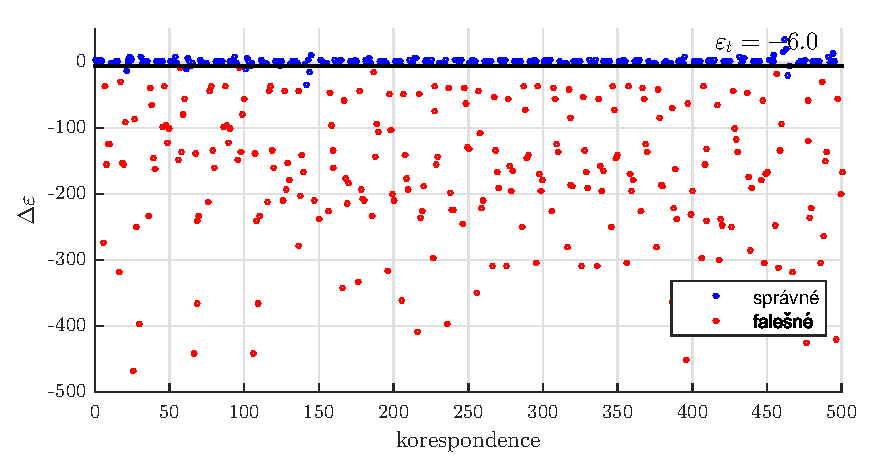
\includegraphics[width = \textwidth]{epsilon1.eps}
\caption[Změna kritéria korespondencí třídy \textbf{9G}.] {Graf $\Delta\varepsilon$ pro prvních 500 korespondencí třídy \textbf{9G}. Správné a špatné korespondence oddělíme prahem $\varepsilon_t = -9.0$. Výsledná oddělitelnost $S = 0.949$.}
\label{fig: epsilon1}
\end{figure}

\begin{figure}[htps]
\centering
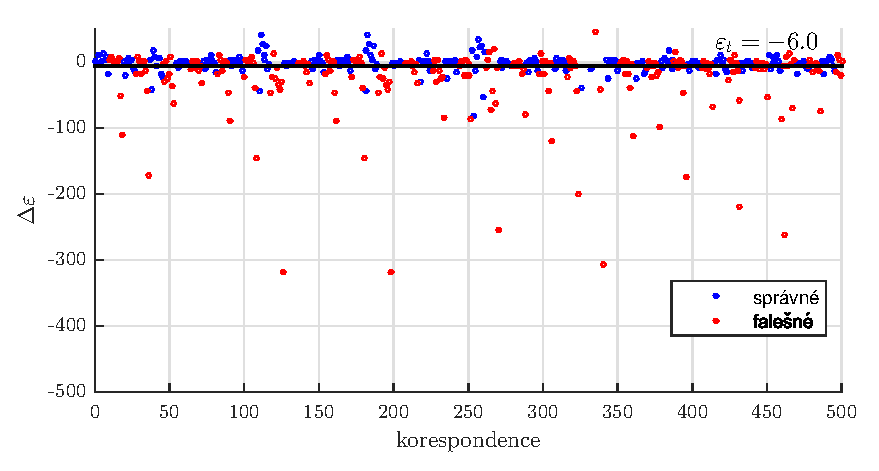
\includegraphics[width = \textwidth]{epsilon2.eps}
\caption[Změna kritéria korespondencí třídy \textbf{7D}.]{Graf $\Delta\varepsilon$ pro prvních 500 korespondencí třídy \textbf{7D}. Třídění korespondencí podle prahu $\varepsilon_t = -6.0$ nevede ke uspokojivému výsledku. Výsledná oddělitelnost $S = 0.594$.}
\label{fig: epsilon2}
\end{figure}

\clearpage